% arara: xelatex: {shell: yes}
% arara: makeglossaries
% arara: bibtex
% arara: xelatex: {shell: yes}
% arara: xelatex: {shell: yes}

% options:
% hidelinks remove colour boxes around hyperlinks
\documentclass[thesis=M,czech,hidelinks]{FITthesis}[2019/12/23]

% \usepackage{subfig} %subfigures
% \usepackage{amsmath} %advanced maths
% \usepackage{amssymb} %additional math symbols

\usepackage[utf8]{inputenc}

\usepackage{dirtree} %directory tree visualisation

% list of acronyms
\usepackage[acronym,nonumberlist,toc,numberedsection=autolabel,nomain]{glossaries}
\iflanguage{czech}{\renewcommand*{\acronymname}{Seznam pou{\v z}it{\' y}ch zkratek}}{}
\makeglossaries

% change typography
\usepackage{fontspec}
\setmonofont[Scale=MatchLowercase]{Fira Code}
\setmainfont[Scale=MatchLowercase]{Lora}
\renewcommand{\baselinestretch}{1.2}

% paragaphs indent
\DisemulatePackage {parskip}
\RequirePackage [parfill] {parskip}

% list padding
\usepackage{enumitem}

% WIP background color
\usepackage{pagecolor}
%\pagecolor{lightgray}

% footnote position
\usepackage[bottom]{footmisc}

% images fullscreen
\usepackage[export]{adjustbox}

% source code
\usepackage{minted}
\setminted{baselinestretch=1}

% refactor section
\definecolor{COLOR_REFACTOR}{HTML}{8e44ad}
\newenvironment{REFACTOR}{\par\color{COLOR_REFACTOR}}{\par}

% figure, table captions are bold
\usepackage[labelfont=bf]{caption}

% highlighter
\usepackage{longfbox}
\makeatletter
\newdimen\@tempdimd
\makeatother
\fboxset{rounded,background-color=\#D8DEE9,border-width=0em,padding={0.3em, 0.5em}}%

% import PDF assignment
\usepackage{pdfpages}
\usepackage{wasysym}
\usepackage{csquotes}

% custom envs
\newenvironment{ul}{
   \begin{itemize}
      \setlength{\itemsep}{0.1em}
      \setlength{\parskip}{0.1em}
      }{
   \end{itemize}
}

\newenvironment{ol}{
   \begin{enumerate}
   }{
   \end{enumerate}
}

\newenvironment{dl}{
   \begin{description}
      \setlength{\itemsep}{0.2em}
      \setlength{\parskip}{0.2em}
      }{
   \end{description}
}

\newcommand{\chaptersummary}[1]{
   \begin{longfbox}[
      padding=1em,
      background-color=white,
      border-width=1pt,
   ]
   \textbf{V dané kapitole:}
   #1
   \end{longfbox}
}
\newcommand{\TODO}[1]{\lfbox[background-color=\#ff0000]{TODO: #1}}
%\newcommand{\h}[1]{\texttt{#1}}
\newcommand{\h}[1]{\lfbox{\texttt{#1}}}
\newcommand{\g}[1]{\gls{#1}}

% change \gls from FULL_NAME (ABBR) -> ABBR (FULL_NAME)
\renewcommand{\acrfullformat}[2]{#2\space(#1)}

% % % % % % % % % % % % % % % % % % % % % % % % % % % % % % % % % % %
% % % % % % % % % % % % % % % % % % % % % % % % % % % % % % % % % % %

\department{Katedra softwarového inženýrství}
\title{Informační systém pro správu projektů v~architektuře mikroservis}
\authorGN{Sergey} %author's given name/names
\authorFN{Dunaevskiy} %author's surname
\authorWithDegrees{Bc. Sergey Dunaevskiy} %author's name with academic degrees
\author{Sergey Dunaevskiy} %author's name without academic degrees
\supervisor{Ing. Michal Valenta, Ph.D.}
\acknowledgements{TODO}
\abstractCS{Tato diplomová práce se zabývá návrhem a implementací informačního systému v architektuře mikroslužeb na základě existující bakalářské práce.
Cílem je přepsat původní architekturu, automaticky otestovat a zajistit kontejnerizaci.
Na základě analýzy oblasti mikroslužeb byly vybrány a adaptovány vhodné varianty pro server i klienta.
Vzhledem k rozsahu práce původní funkionalita byla částečně přenesena do budoucího rozvoje.
V závěru je nové řešení porovnáno s původním a zhodnocen výsledek.
}
\abstractEN{This master's thesis deals with designing and implementing an information system described in the existing bachelor's thesis in microservices architecture.
The goal is to rewrite the original architecture, automatically test and ensure containerization.
Based on the analysis of the area of microservices, suitable variants of the architecture were chosen and adapted.
Due to the scope of the work, some functionality was partially transferred to future development.
In conclusion, the new solution is compared with the previous, and the result is evaluated.
}
\placeForDeclarationOfAuthenticity{V~Praze} %where you have signed the declaration
\keywordsCS{architektura, mikroslužby, server, klient, javascript, nodejs, nextjs, správa projektů}
\keywordsEN{architecture, microservices, server, client, javascript, nodejs, nextjs, project management}
\declarationOfAuthenticityOption{4} %select as appropriate, according to the desired license
\website{https://github.com/dunaevskiy/thesis-masters} %optional URL (remove entirely if you have no URL for this thesis)


\begin{document}

   \newacronym{ACID}{ACID}{atomicity, consistency, isolation, durability}
\newacronym{AJAX}{AJAX}{asynchronous javascript and xml}
\newacronym{API}{API}{application programming interface}
\newacronym{CSS}{CSS}{cascading style sheet}
\newacronym{DOM}{DOM}{document object model}
\newacronym{ES6}{ES6}{ECMAScript 6}
\newacronym{ESB}{ESB}{enterprise service bus}
\newacronym{FIT}{FIT}{Fakulta informačních technologií}
\newacronym{FaaS}{FaaS}{function as a service}
\newacronym{GUI}{GUI}{graphical user interface}
\newacronym{HTML}{HTML}{hypertext markup language}
\newacronym{HTTP}{HTTP}{hypertext transfer protocol}
\newacronym{IDE}{IDE}{integrated development environment}
\newacronym{ID}{ID}{identity}
\newacronym{IIFE}{IIFE}{immediately invoked function expression}
\newacronym{IP}{IP}{internet protocol}
\newacronym{IS}{IS}{informační systém}
\newacronym{IoT}{IoT}{internet of things}
\newacronym{JSON}{JSON}{javascript object notation}
\newacronym{JS}{JS}{JavaScript}
\newacronym{MA}{MA}{monolithic architecture}
\newacronym{MSA}{MSA}{microservices architecture}
\newacronym{MS}{MS}{microservice}
\newacronym{ORM}{ORM}{object relational mapping}
\newacronym{REST}{REST}{representational state transfer}
\newacronym{RPC}{RPC}{remote procedure call}
\newacronym{SA}{SA}{serverless architecture}
\newacronym{SOA}{SOA}{service oriented architecture}
\newacronym{SQL}{SQL}{structured query language}
\newacronym{SSG}{SSG}{static generation}
\newacronym{SSR}{SSR}{server side rendering}
\newacronym{TS}{TS}{TypeScript}
\newacronym{UAT}{UAT}{user acceptance testing}
\newacronym{UI}{UI}{user interface}
\newacronym{URI}{URI}{uniform resource identifier}
\newacronym{UX}{UX}{user experience}
\newacronym{VCS}{VCS}{version control system}
\newacronym{XML}{XML}{extended markup language}
\newacronym{ČVUT}{ČVUT}{České vysoké učení technické}


   \begin{introduction}
      % FINAL, CHECKED

Architektura aplikací tvoří nedílnou součást každého vývoje.
Její náročnost je variabilní v závislosti na typu, složitosti, frekventovanosti použití a dalších parametrech aplikace.
Zpravidla čím menší nároky se na výsledek kladou, tím je navrhovaná architektura primitivnější, aby se ušetřilo na nákladech během vývoje a provozu aplikace.
Komplexnější požadavky však potřebují pro svůj provoz zajistit stabilní prostředí, které se definuje například stabilitou aplikace, způsobem opravy neočekávaných chyb, rychlosti odezvy apod.
Všechny tyto aspekty je mnohdy složité řešit najednou a přirozeně se rozdělují na menší atomické celky, jež by se daly spravovat samostatně.

Koncept mikroslužeb vznikl přibližně před 10 až 15 lety.
Explicitně, jako pojem, byl zmíněn až v roce 2011 v rámci popisu stylu architektury, se kterou se tehdy experimentovalo~\cite{msabegin}.
Prudký růst zájmu o \g{MSA} a mikroslužby celkově (dle statistických údajů Google Trends) byl zaznamenán v listopadu 2014 a začátku roku 2017.
V průběhu roku 2019 dosahoval největší popularity dle relativních počtů vyhledávání~\cite{googletrendsmsa}.
Aktuálně \g{MSA} zůstává velice frekventovaným trendem~\cite{googletrendsmsa}, z tohoto důvodu lze danou architekturu předpokládat za stále využívanou nebo alespoň jevící zájem u určitého množství lidí.

Jelikož daný koncept je poměrné mladý, tak je málo pravděpodobné, že byl plně prozkoumán.
Představuje potenciální oblast pro experimentování a zdokonalování, modifikaci a odvozování jiných, nezávislých vývojových praktik.
Průzkum takových skutečností se nejlépe ověřuje v praxi, v daném případě budou vhodné středně velké aplikace s teoreticky neomezenou možností rozvoje.
Jako příklad takové struktury může být \g{IS} pro správu projektů v akademických institucích.

\clearpage



\section{Cíl práce}\label{sec:cil-prace}
Cílem této diplomové práce je primárně průzkum \g{MSA} se subjektivní úvahou o různých přístupech, technikách a myšlenkách týkajících se daného tématu.
Samostatné části budou věnovány zpracováním databázových transakcí u serverové části a mikroslužbám straně klienta.

Nabyté znalosti se uplatní v praxi ve formě \g{IS} pro správu projektů, který byl navržen a implementován jako prototyp monolitické architektury v bakalářské práci \uv{Informační systém pro správu studijních projektů}~\cite{bachelorthesis}.
I když tento systém bude brán jako stěžejní pro uplatnění znalostí o architektuře a bude uskutečněn přechod z monolitické architektury na architekturu mikroslužeb, tak za cíl není kladeno tento projekt výrazně zlepšit z uživatelského hlediska nebo uvést do provozu v době dokončení diplomové práce.
Postupovat se bude inkrementálně – nejdřív se implementuje nejdůležitější, nezbytná osnova a zbylá funkcionalita bude dokončena dle časových možností, případně uvedena v seznamu pro další rozvoj.

Větší část analýzy a specifikace uvedené v bakalářské práci~\cite{bachelorthesis} bude převzata, některé aspekty však budou explicitně zaktualizovány a popsány v kapitolách \hyperref[ch:analysis]{Analýza předchozí práce} a \hyperref[ch:specification]{Specifikace}, protože mohou způsobovat nevhodný dopad – bezpečnost, nevyhovující funkcionalita apod.

Konečným výstupem bude především popis subjektivně prozkoumané oblasti \g{MSA} sloužící jako rychlý přehled architektury mikroslužeb s případnými dodatečnými materiály, zrefaktorovaná verze \g{IS}, jež je převedena z monolitické architektury na architekturu mikroslužeb, a dodaná příručka vývojáře.
V rámci implementace bude zdokonaleno testování a nasazování výsledné služby.


\newpage



\section{Struktura}\label{sec:struktura}

\textbf{Kapitola 1} se věnuje stručné analýze výsledků předchozí práce, definuje silné a slabé stránky a navrhuje body pro zlepšení, zejména pro \g{MSA}.

\textbf{Kapitola 2} se zabývá obecným zkoumáním problematiky \g{MSA} a typickými situacemi, které se potenciálně mohou řešit během implementace systému s využitím \g{MSA}\\na~straně serveru i klienta.

\textbf{Kapitola 3} rozebírá integraci mikroslužeb s datovými úložišti a problematiku transakčního zpracování v případě oddělených úložišť.

\textbf{Kapitola 4} specifikuje požadavky nového projektu s návazností na analýzu předchozího projektu a souladu se zadáním diplomové práce.

\textbf{Kapitola 5} obsahuje analýzu a implementaci serverové části \g{IS} v \g{MSA} s uplatněním informací popsaných v kapitolách analýzy \g{MSA}.

\textbf{Kapitola 6} obdobně, jako v případě předchozí kapitoly, obsahuje analýzu a implementaci klientské části aplikace.

\textbf{Kapitola 7} se věnuje popisu zlepšeného testování obou částí \g{IS}.

\textbf{Kapitola 8} se zabývá kontejnerizací a nasazováním \g{IS}.

\textbf{Kapitola 9} je věnována nedostatkům aktuálního řešení a potenciálnímu budoucímu rozvoji.

\textbf{Kapitola 10} porovnává původní monolitický prototyp s novou realizací systému a uvádí přínosy a nevýhody přechodu.

V závěrečné kapitole je zhodnocen výsledek a dosažení předem stanovených cílů a splnění zadání diplomové práce.

V přílohách a na přiloženém médiu jsou uvedeny zdrojové kódy všech částí \g{IS}, dokumentace pro vývojáře a jiné dodatečné materiály.

   \end{introduction}

   % FINAL, CHECKED

\chapter{Analýza předchozí práce}\label{ch:analysis}

\chaptersummary{
   \begin{ul}
      \item analýza posudků vedoucího a oponenta předchozí práce,
      \item analýza popsaných možností rozvoje systému,
      \item zkoumání silných a slabých stránek implementovaného systému,
      \item revize změn na fakultě z hlediska správy projektů.
   \end{ul}
}

Tato diplomová práce navazuje na bakalářskou práci z roku 2019~\cite{bachelorthesis} a využívá jak analýzu/výsledky popsané v práci samotné, tak i přílohy (zejména zdrojový kód serverové aplikace, klientské aplikace a vývojářské a uživatelské dokumentace).
Pro implementování daného systému v \g{MSA} a zajištění kvality výsledku je provedena opakovaná analýza problematiky a korekce potřebných oblastí.



\section{Potenciální možnosti rozvoje systému}



\subsection{Posudky}
Ze závěrečných posudků vedoucího a oponenta bakalářské práce je nutno vyčlenit několik významných bodů pro zlepšení.

\begin{ul}
   \item
   \textbf{Neúplná či nedostatečně propracovaná dokumentace~\cite{bachelorthesisreportsupervisor}} – je třeba přepracovat poskytnuté dokumentace a doplnit relevantními informacemi – přidat informace o architektuře, způsobu fungování, zřetelnější práci s databází a použité technologie.
   \clearpage

   \item
   \textbf{Velice stručně popsané testování~\cite{bachelorthesisreportreviewer}} – v poskytnutém systému je velice málo automatizovaných testů a probíhalo zejména manuální testování~\cite{bachelorthesis} – některé části se dají dobře začlenit do vývojového cyklu s automatickým spouštěním.

   \item
   \textbf{Nebylo popsané konkrétní určení informačního systému~\cite{bachelorthesisreportreviewer}} – informační systém od začátku nebyl cílený pro konkrétního spotřebitele.
\end{ul}

Zároveň během obhajoby bakalářské práce bylo nabídnuto zvážit správu a ukládání projektu ve \g{VCS} git místo manuálního ukládání v NoSQL databázi (MongoDB).
To by mohlo zredukovat množství potřebného kódu a snížilo spotřebu fyzické paměti (jednotlivé snímky odevzdaných projektů by se neduplikovaly, ale ukládaly jako git značky\footnote{git tags}).



\subsection{Možnosti rozvoje}

Bakalářská práce navrhuje rozvoj 2 hlavními směry - obecné univerzální zdokonalování a rozvoj se zaměřením na \g{FIT} \g{ČVUT}~\cite{bachelorthesis}.
Jelikož daná práce se soustředí především na \g{MSA}, tak rozvoj se zaměřením na fakultu bude považován za sekundární.
V předchozí práci bylo nabídnuto několik bodů pro rozvoj~\cite{bachelorthesis}.


\begin{ul}
   \item
   \textbf{Podpora internacionalizace a lokalizace} – aplikace poskytuje pouze anglické rozhraní.
   Nepoužívá se žádný framework nebo knihovna, která by napomáhala snadné správě překladů.

   \item
   \textbf{Hromadné zakládání projektů} – neexistuje způsob hromadného zakládání projektů, i když dle předchozí analýzy by byl prospěšný.

   \item
   \textbf{Serverová implementace snímků} – nedokončená funkcionalita pro odevzdávání jednotlivých iterací projektů.

   \item
   \textbf{Nepříznivé scénáře \g{API} dotazů} – v případě pádu serveru a neočekávané \g{API} odpovědi často chybí uživatelsky přijatelné oznámení/zpracování.

   \item
   \textbf{Nové interprety obsahu} – jedná se o omezený výběr vytvářených typů obsahů.

   \item
   \textbf{Propracovaná integrace se službami třetích stran} – funkcionalita propojení fakultních služeb pro známkování, autorizaci apod.

   \item
   \textbf{Analýza využití systému a aktualizace \g{UX}} – bez produkčního prostředí (nebo jiného dlouhodobého uživatelského testování) nebylo možné získat daná data.

   \item
   \textbf{Optimalizace stávajícího systému} – různorodá optimalizace předchozího \g{IS}.
\end{ul}



\subsection{Revize kódu}

\begin{ul}
   \item
   \textbf{\g{IS} není plně kontejnerizovaný} – \g{IS} není plně převeden na kontejnery, může být zdlouhavější start projektu, to se v pozdějších fázích odrazí i na předpokládané škálovatelnosti služby.

   \item
   \textbf{Monolitická struktura aplikace} – jakákoliv úprava vyžaduje editaci celého systému, není možné pohodlně měnit jednotlivé části aplikace.

   \item
   \textbf{Staré a vyřazené z provozu knihovny} – v klientské React aplikaci se nachází starší knihovny, jež musí být aktualizovány (bezpečnost, nová funkcionalita, \dots).
   Rovněž je možné uplatnit nový způsob psaní React aplikací – s React Hooks.

   \item
   \textbf{Konfigurace a zbytečné oddělování prostředí} – bude potřeba zvážit konfiguraci přes \texttt{.env} soubory a odstranit rozdělení způsobů startu aplikace dle prostředí.

   \item
   \textbf{Struktura projektu, architektura} – některé prvky, struktura složek a návrh architektury se zdají být v mnoha případech zbytečné a přispívají nečitelnosti.
\end{ul}



\section{Silné stránky}
Z hlediska pozitivních prvků poskytnuté implementace lze vytknout několik skutečností:

\begin{ul}
   \item
   \textbf{JavaScript, TypeScript a Node.js} – serverová a klientská část aplikace jsou psány v jazyce JavaScript (případně TypeScript), je to výhodné z hlediska udržování systému.

   \item
   \textbf{Knihovna Next.js} – klientská část je psána v jedné z moderních knihoven Next.js s podporou \g{SSR} a \g{SSG}~\cite{nextjs}.

   \item
   \textbf{Dynamicky generovaný obsah projektů} – způsob tvorby obsahu stránky připomíná implementaci mikroslužeb na straně klienta.

   \item
   \textbf{Kontejnerizace aplikací} – databáze jsou poskytovány s pomocí služby Docker a potřebují minimum konfigurací.
\end{ul}



\section{Alternativní systémy správy projektů na fakultě}

Vzhledem k relativně dlouhé době (3 roky) od dokončení bakalářské práce je potřeba provést stručnou aktualizaci seznamů alternativních řešení pro správu projektů na fakultě.
U předchozích systémů fungujících na fakultě (v návaznosti na rešerši způsobů správy projektů na \g{FIT} \g{ČVUT}~\cite{bachelorthesis}) je možné zaznamenat následující změny:

\begin{ul}
   \item
   \textbf{Project/SwinPro} – provoz aplikace je ukončen ke dni 1. 10. 2021 a veškerá data jsou dostupná pouze na požádání prostřednictvím osobního e–mailu~\cite{swinpro}.
   \item
   \textbf{Roundcube\footnote{Webmail}} – byl nahrazen službou Microsoft 365 s vlastními e–mailovými schránkami~\cite{emailsfitcvut}.
   \item
   \textbf{Microsoft Teams} – během vzdálené výuky některé předměty využily funkcionality služby Microsoft Teams pro vytvoření požadavku na odevzdání souboru semestrální práce\footnote{Jedná se o osobní zkušenost z předmětů NI–MPI a NI–PIS}.
   \item
   \textbf{Studentský odevzdávací systém} – vznikl nový portál pro studentské projekty.
   Jelikož se jedná o komplexní řešení, bude rozebrán samostatně v následující podkapitole.
\end{ul}



\subsection{Studentský odevzdávací systém (SOS)}

\textbf{Autor:} kolektiv autorů (závěrečné práce)\newline
\textbf{Analyzovaná verze:} 0.2.3-alpha\newline
\textbf{Datum analýzy:} 31.~10.~2021\newline
\textbf{URL:} \url{https://sos.fit.cvut.cz/}

\begin{figure}[htbp]
   \centering
   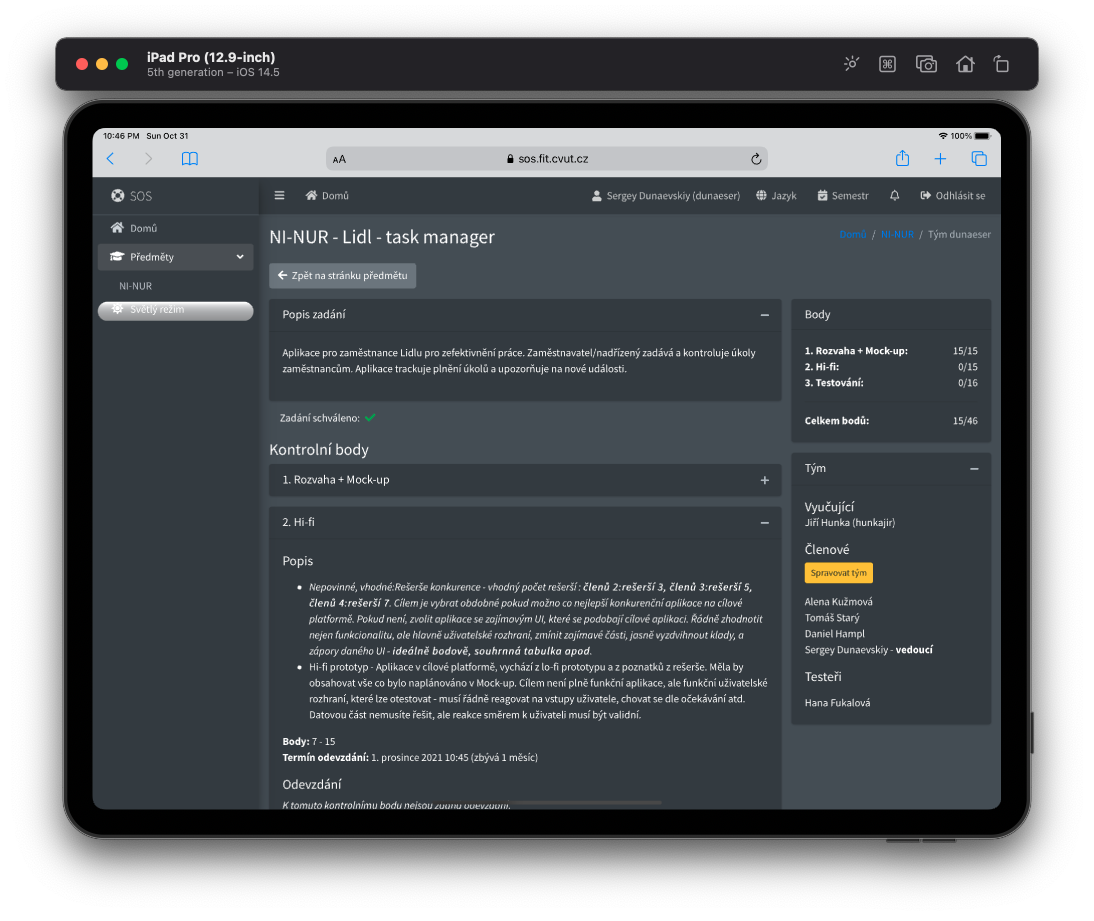
\includegraphics[max width=\textwidth]{assets/analysis-sos-portal}
   \caption[Studentský odevzdávací systém – ukázka detailu projektu]{Studentský odevzdávací systém – ukázka detailu projektu z pohledu studenta}\label{pic:sos-portal}
\end{figure}


Studentský odevzdávací systém je relativně nový portál – nachází se v alpha verzi a využívá se například v předmětu NI-NUR.
Konceptuálně je myšlen jako univerzální systém pro všechny možné projekty, které vyžadují iterativní odevzdávání souborů a obdržení ohodnocení za odevzdanou práci.
Z pohledu studenta lze vytvořit návrh projektu, který může, ale nemusí být schválen vyučujícím, bohužel nelze vytvářet nekontrolované projekty pro vlastní účely.
Následuje tvorba projektu mimo systém a odevzdávání výsledků v podobě samostatných souborů s případným komentářem.
Započatý projekt nelze přerušit ze strany studenta.
Daný systém se v mnoha ohledech podobá \g{IS}, který byl analyzován v předchozích podkapitolách.

\textbf{Společné rysy}

\begin{ul}
   \item
   \textbf{Iterativní odevzdávání projektu} – založený projekt se odevzdává v iteracích (kontrolních bodech), které mohou být okomentovány a ohodnoceny ze strany vyučujícího.
   \item
   \textbf{Odpovědná osoba} – existuje role (vyučující), která dokáže ohodnotit kontrolní bod určitých počtem bodů.
\end{ul}


\textbf{Výhodné prvky}

\begin{ul}
   \item
   \textbf{Nahrávání souborů} – v rámci iterace lze nahrávat libovolné soubory.
   \item
   \textbf{Integrace s fakultními systémy} – \g{IS} je víc přizpůsobený pro fakultní účely.
   \item
   \textbf{Tmavé rozhraní} – \g{UI} má volitelný tmavý režim, viz obrázek~\ref{pic:sos-portal}.
   \item
   \textbf{Jazyky} – \g{UI} je poskytováno v anglickém a českém jazyku s libovolným přepínáním.
\end{ul}


\textbf{Negativní prvky}

\begin{ul}
   \item
   \textbf{Restrikce zakládání projektů} – studenti nemohou zakládat vlastní, nezávislé projekty, musí spadat pod určitý předmět.
   Nelze založit a spravovat víc projektů.
   \item
   \textbf{Nelze založit víc projektových rolí} – projektové role i pro vedoucího projektu jsou omezeny na členy týmu a testery, nelze přidat libovolnou roli.
   \item
   \textbf{Neintuitivní rozhraní} – některé prvky uživatelského rozhraní nejsou intuitivně pochopitelné (subjektivně) a při kritické změně nevyžadují potvrzení.
\end{ul}

   \chapter{Mikroservisní architektura - Obecný úvod}\label{ch:msa-intro}

\chaptersummary{
   \begin{ul}
      \item obecné informace o architektuře a proč je důležitá,
      \item porovnání vybraných architektur – \g{MSA}, \g{MS} a \g{SOA},
      \item typy dekompozice specifikace na \g{MSA} architekturu,
      \item komunikace mezi mikroslužbami a řešení závislostí,
      \item testování a validace mikroslužeb,
      \item nasazení mikroslužeb na server a základní monitorování,
      \item krátký úvod do \g{MSA} na straně webového klienta.
   \end{ul}
}


Softwarovou architekturu jako pojem je těžké exaktně definovat, každý vývojář k ní může přistupovat a vnímat jinak.
Obecně může být popsána jako jistý řád a pravidla, vzniklá následekem mnoha rozhodnutí v průběhu analýzy a vývoje projektu.
Veškerý následující rozvoj by se měl striktně řídit těmito pravidly, aby umožnil dlouhodobě udržovatelný výsledek.
~\cite{softarch}

Vývoj softwaru bez architektury nebo s nepřesně definovanou osnovou může být přínosný v krátkodobé perspektivě nebo z hlediska šetření počátečních nákladů na čas a finanční složky~\cite{softarch}.
V případě dlouhodobého projektu to všas může znamenat hromadění technického dluhu ~\cite{archoworthit}.
Dle článku~\cite{archoworthit} přínos architektury lze vizuálně znázornit grafem~\ref{fig:architecture-line}, kde je uvedena komulativní funkcionalita v závislosti čase spotřebovaným projektem.
Používání architektury ze začátku způsobuje zpomalení vývoje, ale od jisté hranice výhody se stává přínosnou a urychluje rozvoj.
Tento předpoklad však funguje pouze v případě, že se jedná o dobře zvolenou a popsanou architekturu (v textové nebo digramové podobě), která má pozitivní vliv a je dostatečně ohebná~\cite{archoworthit}.


\begin{figure}[htbp]
   \centering
   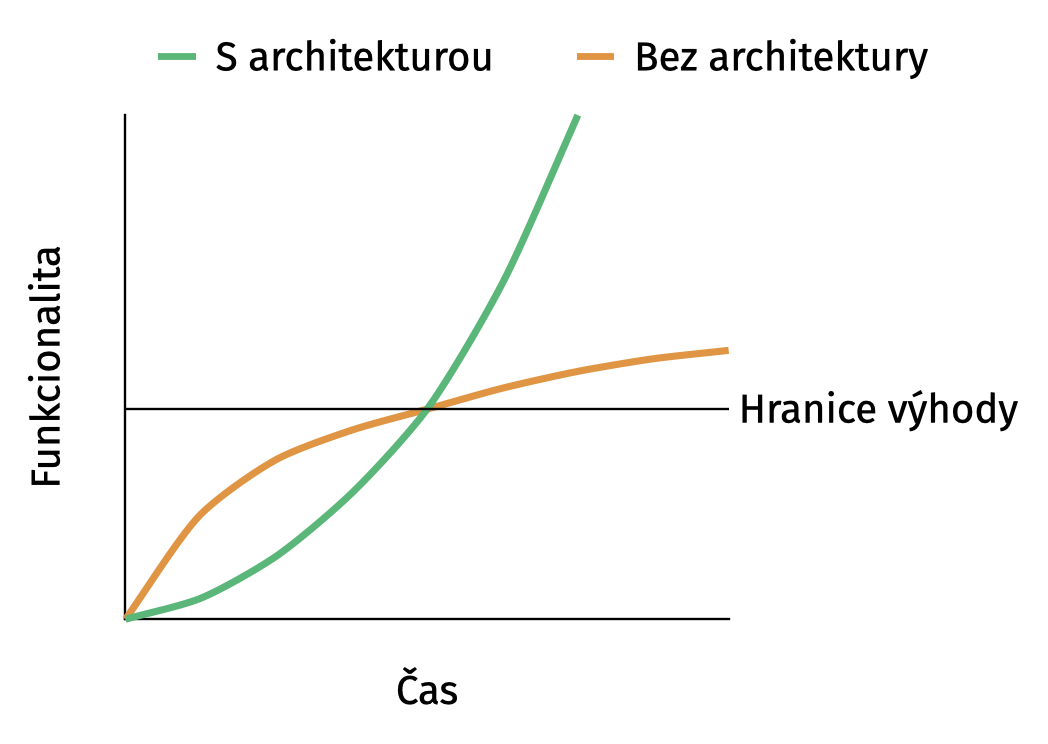
\includegraphics[max width=\textwidth]{assets/draft-architecture-line}
   \caption{Bod přínosu dodržování architektury~\cite{archoworthit}}\label{fig:architecture-line}
\end{figure}


Ačkoli neexistuje přesná definice architektury, existují nějaké šablony architektury, které jsou vhodné pro vývoj aplikací.
Jejich volba a případná adaptace vyžaduje pochopení konečného cíle požadovaného výsledku~\cite{softarch}.
V návaznosti na zadání diplomové práce v dané kapitole bude popisována především \g{MSA} a bude porovnávana s jinými architekturami, které by ji potenciálně mohly nahradit.
Tyto vybrané architektury – \g{MA}, \g{SOA}\footnote{též architektura orientovaná na služby}, \g{SA} – budou zkoumány vzhledem k přístupu k určitým aspektům, poskytovaným možnostem a výhodám a nevýhodám vůči \g{MSA}.
Vzhledem k dříve použitému jazyku TypeScript/JavaScript budou i mikroservisy zkoumány se zaměřením na tento jazyk, případně Node.js prostředí.


Než se začne s konkrétním porovnáním, je třeba definovat jeden společný pojem všech 3 architektur – službu.
Služba v této práci je chápána jako atomicky fungující celek, z větší části nezávislý na ostatních – soustředí se na konkrtétní funkcionalitě (nebo skupině funkcionalit), má přístup k databázovému úložišti a veškerá komunikace probíhá přes striktně definované rozhraní (vizualizaci takové služby je možné vidět na obrázku~\ref{fig:service-abstract}).
Může fungovat jako celek poskytující, přijímající a zpracovávající nebo předávající datové zprávy.
Jakýkoliv jiný vliv, než přes dohodnuté rozhraní, je ignorován a musí být ideálně eliminován.
Rozhraní takové služby může být popsáno s pomocí samostatné dokumentace nebo dokumentovaného kódu.


\begin{figure}[htbp]
   \centering
   
\includegraphics[max width=\textwidth]{assets/draft-service}
   \caption{Abstraktní znázornění služby}\label{fig:service-abstract}
\end{figure}


Kvůli nejednoznačnosti pojmu \h{architektura} nejspíš existuje nespočetné množství modifikací a adaptací výše uvedených architektur (\g{MA}, \g{SOA}, \g{MSA}, \g{SA}), proto se bude předpokládat, že se jedná o takto definované instance:

\begin{dl}
   \item[\g{MA}] – jednoprocesový program atomické povahy – nelze z něho jednoduše vyčlenit funkční celky, které by se daly beze změn využívat v jiných programech.
   Obsahuje globální jednorázové připojení k datovému zdroji, které se provádí během startu.
   Takový program je sám o sobě službou.
   \item[\g{SOA}] – jednoprocesový program s interním rozdělením na služby, které mezi sebou komunikují přímo, nebo přes \g{ESB} – sběrnicí určenou pro centralizaci komunikace mezi službami.
   Vazba na datový zdroje může, ale nemusí být jedna (každá služba může mít samostatné připojení).
   \item[\g{MSA}] – několikaprocesový systém služeb organizovaný do větší interně kompatibilní struktury.
   \item[\g{SA}] – architektura aplikace, která postrádá kontinuálně běžící serverový proces a je pouze rozmístěna na \g{FaaS} řešení.
   Jinými slovy funkcionalita není spuštěna v nepřerušovaném prostředí (jako démon), ale je dostupná na požádání.
   Během uživatelského dotazu je vytvořena potřebná instance aplikace, případně navázáno databázové spojení, vykonán požadavek a následně je instance odstraněna.
\end{dl}




Softwarová architektura jako pojem není přesně definována \cite{softarch}

Arichitektura může být popsána jako jistý řád a pravidla, dle kterých je celá aplikace postavena.
Existují nějaké šablony architektury, které jsou vhodné pro vývoj aplikací


V dané kapitole bude popisována především \gls{MSA} a bude porovnávana s jinými architekturami, které by ji potenciálně mohly nahradit.
Tyto vybrané architektury – \gls{MA}, \gls{SOA}\footnote{též architektura orientovaná na služby}, \gls{SA} – budou zkoumány vzhledem k přístupu k určitým aspektům, poskytovaným možnostem a výhodám a nevýhodám vůči \gls{MSA}.



Služba (bez vazby na architekturu) je chápána jako atomicky fungující celek, z větší části nezávislý na ostatních – soutředí se na konkrtétní funkcionalitu, má vlastní databázi (nebo schéma) s výhradným přístupem a veškerá komunikace probíhá přes striktně definované rozhraní.
Jakýkoliv jiný vliv, než přes dohodnuté rozhraní, musí být eliminován.

Jelikož existuje nespočetné množství modifikací výše uvedených architektur, bude se předpokládat, že se jedná o takto definované instance:


%https://www.ibm.com/cloud/learn/soa#toc-soa-vs-mic-BjTfju28

\begin{dl}
   \item[\gls{MA}] – jednoprocesový program atomické povahy – nelze z něho jednoduše vyčlenit funkční celky, které by se daly beze změn využívat v jiných programech.
   Obsahuje globální jednorázové připojení k databázi, které se provádí během startu programu a kontroluje aktuální stav migrací (případně vykonává chybějící).
   \item[\gls{SOA}] – jednoprocesový program s interním rozdělením založeným na \gls{ESB} – sběrnicí určenou pro centralizaci komunikace mezi službami.
   Jednotlivé služby tvoří samostatně fungující moduly, jež veškerou komunikaci provádí skrz přesně definované rozhraní \gls{ESB}.
   Obdobně, jako u \gls{MA} existuje jedno
   \item[\gls{MSA}] –
   \item[\gls{SA}] – architektura aplikace, která postrádá neustále běžící serverový proces a je pouze rozmístěna na \gls{FaaS} řešení.
   Jinými slovy funkcionalita není spuštěna v nepřerušovaném prostředí (jako démon), ale je dostupná na požádání.
   Při dotazu (například REST) je vytvořena potřebná instance aplikace, případně navázáno databázové spojení, vykonán požadavek a následně je instance odstraněna.
   Taková aplikace nemůže být stavová v obvyklém slova smyslu.
   Kvůli průběhu zpracování se rovněž nehodí pro náročné aplikace. \TODO{zdroj}
\end{dl}

Pro porovnání architektur bylo vybráno několik klíčových pojmů, které mohou během návrhem a implementací programu mít nějvětší vliv na rozhodování o výběru architektury.

+- MA OR 29


\begin{dl}
   \item[Datové úložiště] – využití persistentního úložiště (SQL/NoSQL databáze) pro zápis a čtení informací.
   Počáteční inicializace databáze, vytvoření struktury, migrace
\end{dl}
\begin{ul}
   \item \gls{MA} – není náročná pro testování.
   \item \gls{SOA} – rovněž může být testována
   \item \gls{MSA} – plnohodnotné testování celé struktury vyžaduje její nasazení na server.
\end{ul}

\begin{dl}
   \item[Nezávislost] – popis
\end{dl}
\begin{ul}
   \item \gls{MA} – něco umí
   \item \gls{SOA} – něco umí
   \item \gls{MSA} – něco umí
\end{ul}

\begin{dl}
   \item[Radikální změny] – složitost změny nebo přidání business logiky do aplikace, která by měl dopad na větší část dosavadní aplikace.
\end{dl}
\begin{ul}
   \item \gls{MA} –
   Z hlediska datového úložiště bude potřeba dělat pouze jednu migraci
   \item \gls{SOA} – něco umí
   \item \gls{MSA} – něco umí
\end{ul}

\begin{dl}
   \item[Tolerace chyb] – popis
\end{dl}
\begin{ul}
   \item \gls{MA} – něco umí
   \item \gls{SOA} – něco umí
   \item \gls{MSA} – něco umí
\end{ul}

\begin{dl}
   \item[Komunikační latence] – popis
\end{dl}
\begin{ul}
   \item \gls{MA} – něco umí
   \item \gls{SOA} – něco umí
   \item \gls{MSA} – něco umí
\end{ul}

\begin{dl}
   \item[Škálování] – popis
\end{dl}
\begin{ul}
   \item \gls{MA} – něco umí
   \item \gls{SOA} – něco umí
   \item \gls{MSA} – něco umí
\end{ul}

\begin{dl}
   \item[Konzistence] – popis
\end{dl}
\begin{ul}
   \item \gls{MA} – něco umí
   \item \gls{SOA} – něco umí
   \item \gls{MSA} – něco umí
\end{ul}

\begin{dl}
   \item[Nasazení] – popis
\end{dl}
\begin{ul}
   \item \gls{MA} – něco umí
   \item \gls{SOA} – něco umí
   \item \gls{MSA} – něco umí
\end{ul}

\begin{dl}
   \item[Testování] – schopnost psaní automatizovaných testů, které se vyplní při spuštění aplikace.
\end{dl}
\begin{ul}
   \item \gls{MA} – něco umí
   \item \gls{SOA} – něco umí
   \item \gls{MSA} – něco umí
\end{ul}

\section{Využití \g{MSA} pro modelování světa}\label{sec:msa-model-of-world}

Pro člověka nejspíš neexistuje nic přirozenějšího, než prostředí, ve kterém se pohybuje a kterému rozumí – od osobních věcí a proseců, jež musí vykonávat, až po uspořádání světa – město, stát, planeta, politické a sociální vztahy, komunikace s institucemi a interakce s rodinou.

Všechny tyto činnosti můžeme popsat pomocí subjektů – samostatných účastníků procesů, rozhraní, které poskytují pro komunikaci, a zpráv\footnote{Zprávou se rozumí informace poskytnutá v samostatné struktuře – například \g{JSON} nebo \g{XML}}, jež se předávají v rámci komunikace.
Každý subjekt je skupinou izolovaných funkcí s různě kompikovanou sadou komunikačních kanálů.
Může mít svoje potřeby a může vytvářet podněty pro ostatní subjekty.
Ne každý subjekt je schopen zpracovávat veškerou informaci, která k němu přichází od jiných subjektů.

Daný konecept naprosto přesně napodobuje \g{MSA}.
Jednotlivé subjekty jsou mikroslužby, mají vlastní rozhraní a vysílají informace v přesně definovaných strukturách.
Mohou existovat samostatně, i když jejich smysl existence nemusí existovat.
Zároveň jsou schopny zachytit a zpracovat zprávy, které byly určeny pro jejich použití a formát kterých je popsaný ve vnitřní logice.

V případě mírného zjednodušení se můžeme dostat ke konceptu \g{SOA}.
Subjekty zachovávají způsob komunikace s pomocí zpráv, ale již nejsou samostatní, potenciálně fungující celky, nýbrž moduly jednoho většího bloku.
Komunikace u takové architektury může být centrállně řízena \g{ESB}.\cite{soavsmsa}

Monolitní architektura v provonání se \g{SOA} zjednodušuje i samotné rozdělení do modulů.
Stále se jedná o samostatně fungující celek, ale vnitří struktura už postrádá moduly s odděleným rozhraním komunikace s využitím zpráv.
V rámci modelování světa se dá představit jako interně nedělitelný celek, který pouze poskytuje rozhraní pro komunikaci, tudíž je to subjekt a v rámci \g{MSA} může představovat mikroslužbu.

Na základě výše uvedených informací by logicky bylo nejjednodušší vždy vytvářet pouze \g{MSA} architekturu, protože je pro pochopení nejsnažší kvůli zkušenostem z každodenního života.
Každý subjekt má svoje potřeby (potřeva vytvořit zprávu, potřeba zpracovat příchozí právu) a o zbylé aspekty se nestará.
Problém nastává kvůli komplexnosti takového konceptu.
Jakékoliv rozdělení celku implicitně předpokládá nové náklady pro definování komunikace, které jsou náročné pro představu.
Proto může být nejvýhodnější začít architektorou s nejvíc redukovaným rozdělením – monolitem a dle potřeby měnit hloubku rozdělení.

Navíc při detailním zkoumání ve všech výše uvedených architekturách se dá vypozorovat rekurzivita.
Monolitická aplikace nebo \g{SOA} aplikace může tvořit mikroslužbu v rámci \g{MSA}.
\g{MSA} aplikace může tvořit mikroslužbu jiné \g{MSA} a fungovat jako monolit pro ostatní.

\section{Dekompozice na \g{MSA}}\label{sec:msa-decomposition}

Projekt, u něhož bylo rozhodnuto o \g{MSA}, vyžaduje, jako jeden z kroků před implementací, dekompozici zadání na oblasti, dle kterých budou následně vytvářeny jednotlivé služby.
Stejně jako v případě myšlenky modelování světa, účastníky procesů budou subjekty a jejich rozhraní pro komunikaci, které v případě projektu lze vyčíst specifikace.

Jinými slovy definování konkrétní architektury projektu se dá provádět postupně ve 3 fázích~\cite{msachris} \TODO{OR74} (vizualizace na obrázku~\ref{fig:msa-decomposition-flow}):


\begin{ol}
   \item Definování operací zpracovávaných serverem – na základě specifikace projektu, ve které jsou popsány požadavky očekávané od serverové části aplikace, formulujeme do konkrétních volání – získat, vytvořit, aktualizovat data.
   \item Definování možných služeb – pro dekompozici na konkrétní služby existují dva základní přístupy – rozdělení dle subdomén a prozdělení dle obchodních potřeb~\cite{msachris}, oba přístupy budou stručně popsány v dalších podkapitolách.
   Oba přístupy vychází z navrhnutých volání a přiřazuje je jednotlivým službám.
   \item Definování propojení požadavků se službami a komunikace služeb mezi sebou – prohlubuje definovanou komunikaci mezi službami a vytváří konkrétní interní a externí spoje.
\end{ol}


\begin{figure}[htbp]
   \centering
   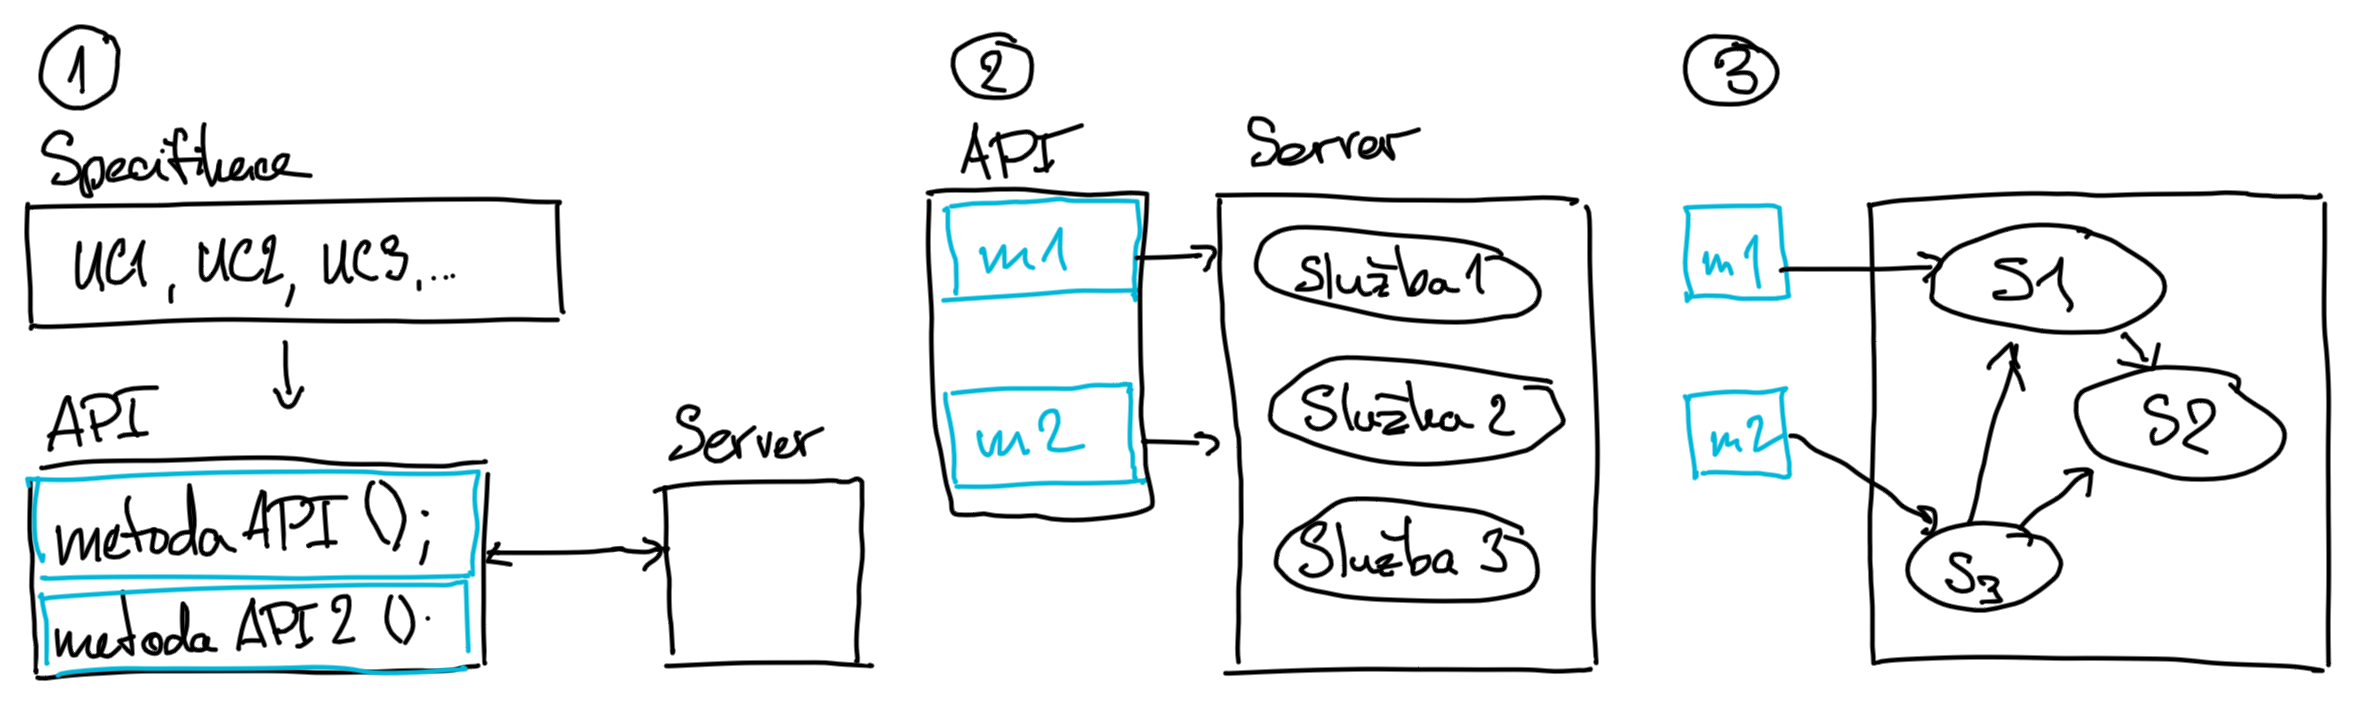
\includegraphics[max width=\textwidth]{assets/draft-decomposition-flow}
   \caption{Tři kroky návrhu \g{MSA}}\label{fig:msa-decomposition-flow}
\end{figure}


V rámci rozdělování operací do konkrétních služeb (stejně jako návrh služeb) mohou pomoci i návrhové vzory týkající se vývoje samotného, jako jsou například:


\begin{dl}
   \item[Princip jedné odpovědnosti] – každá třída musí mít právě jeden důvod, proč se měnit~\cite{srp}.
   V kontextu mikroslužeb se to rovněž vztahuje i na službu samotnou – musí se zabývat pouze jednou subdoménou řešeného problému.
   \item[Vysoká soudržnost] – služba obashuje vše potřebné pro řešení oblasti, za níž je odpovědná~\cite{lchc}.
   \item[Nízká provázanost] – služba může získávat informace z ostatních zdrojů, ale snížená provázanost ulehčuje vývoj~\cite{lchc}.
\end{dl}


Vzhledem k širokému rozsahu dostupných modifikací \g{MSA} je sem možné začlenit mnohem větší spektrum pravidel a doporučení, vždy záleží na aspektech konkrétního zadání.
Některé z nich budou popsány v následujících kapitolách a mohou mít vliv na rozhodnutí spojená s dekompozicí vytvářené funkcionality.



\subsection{Dekompozice dle obchodních potřeb}\label{subsec:msa-decomposition-business}
Dekompozice oblastí dle obchodních potřeb je jednou ze dvou základních možností, jak dokompozici provádět~\cite{msachris}.
Soutředí se na vazbě s architekturou společnosti, neboli něčem, co firmě přináší užitečnou hodnotu~\cite{decompbusiness}.
Uvažujme případ, že o vytvoření \g{MSA} požádala firma, která zpracovává různé druhý objednávek - oblečení, potraviny, sportovní nářadí a spravuje interní pracovníky – stálé zaměstnance a příležitostnou výpomoc.
Z takové struktury by mohlo vzniknout 5 služeb, které by spravovaly:


\begin{ul}
   \item objednávky oblečení,
   \item objednávky potravin,
   \item objednávky sportovního nářadí,
   \item správu zaměstnanců,
   \item správu výpomoci.
\end{ul}



\subsection{Dekompozice dle subdomén}\label{subsec:msa-decomposition-domain}
Dekompozice z hlediska subdomény, která představuje druhý způsob rozdělení, na rozdíl od obchodních požadavků nevnímá architekturu společnosti jako zásadní, i když je nutná, a upřednostňuje logické rozdělování~\cite{decompsubdomain}.
V případě stejného příkladu firmy by dekompozice dle subdomén mohla vypadat následovně:


\begin{ul}
   \item objednávky,
   \item správa pracovníků.
\end{ul}


Takové služby už by nebyly specializované na konkrétním užití a tudíž by mohly být větší nároky na jejich schopnost se přizpůsobovat potřebám \g{IS}.

Typ dekompozice nelze přesně stanovit, je třeba se dívat na všechny potřebné aspekty zkoumané domény a přizpůsobovat dané metody konkrétním situacím~\cite{msachris}.


\section{Závislosti a komunikace}

Mikroservisy jsou vždy nezávislé z hlediska procesů, ale musí udržovat kompatibilní \g{API} s ostatním prostředím.
Takové závislosti se nejlépe kontrolují verzováním jednotlivých mikroservis s pomocí sématického verzování.
Zde je třeba najít konkrétní nástroj pro tuto kontrolu.


- Orchestrace VS Choreografie

\subsection{Komunikace}
- sync/async
- latence
- problém řetězových závislotí


\section{Testování a automatizace}

Daná kapitola se věnuje problematice automatizace testování projektu napsaného v architektuře mikroslužeb s dodaným uživatelským webovým rozhraním.
V rámci testování budeme uvažovat pouze následující kategorie:

\begin{dl}
   \item[Jednotkové testování] – testování nejmenších částí implementace (funkce, třídy aj.),
   \item[Integrační testování] – testování integrací v rámci jedné \g{MS} i mezi \g{MS},
   \item[Funkční testování] – testování funkčnosti bez znalosti interní implementace~\cite{testtypes} dle testovacích scénářů,
   \item[Testování výkonu] – testování systému v předem dané zátěži.
   \item[Testování spolehlivosti] – testování způsobu chování v případech přetížení/výpadku a schopnost se obnovit po výpadku~\cite{testtypes2}.
\end{dl}

V ideálním případě je snaha mít každý automatizovaný typ testování automaticky spouštěný ve správnou chvíli během vývojového cyklu a nasazení sytému.
V případě neexistence možnosti vytvořit automatizaci nebo automacké spouštění, bude potřebný typ testování
Akceptovaným bude rovněž dokumentace s


Existují i další typy testů, jež se mohou automatizovat – testy bezpečnosti, kompatibility, přenositelnosti apod.
V dané práci se jimi zabývat nebude.


\section{Nasazování}\label{sec:msa-deployment}

Nasazení mikroslužeb je jedna ze závěrečných fází vývoje systému, pokrývá široké spektrum možností – rozmístění produkčních balíčků na samostatných fyzických serverech, cloud-řešení, v klasterech, s vyvažováním zátěže, replikací apod.
Daná podkapitola se bude věnovat pouze společným rysům – přípravě pro všechny typy nasazení – a kontejnerizací, jež je vyžadována zadáním diplomové práce.


\subsection{Správa zdrojového kódu}\label{subsec:msa-deployment-code}

Služba, případně mikroslužba, z hlediska chování byla v této práci definována jako samostatný, atomicky fungující celek.
Toto se týká i existence spuštěné instance – musí být schopna existovat samostatně (alespoň z hlediska propojení s ostatními službami).
Taková vlastnost má důležitý dopad na potřebné horizontální škálování a rozložení zátěže v nejvyužívanějších částech systému~\cite{monomulti}.

I přes takové předpoklady samotnou správu zdrojového kódu je možné uspořádat jak do jednoho (monorepozitář) tak i více repozitářů (za předpokladu, že se využívá \g{VCS} git).
Oba přístupy mají své výhody a nevýhody.


\begin{dl}
   \item[Monorepozitář] – existence jednoho repozitáře, kde jednotlivé služby jsou umístěny do vlastních složek.

   \textbf{Výhody}
   \begin{ul}
      \item Celý produkt je uchováván na jednom místě - pro tým to může znamenat lepší podmínky pro testování a vývoj, jelikož mají dostupné všechny vyvíjené častí všemi týmy~\cite{monomulti}.
      \item V případě refaktorování nebo testování systému je možné vše provádět na~jednom místě~\cite{monomulti}.
      \item Vývojové prostředí je možné nastavit tak, že všechny služby budou sdílet stejnou konfiguraci (kontrola kvality kódu, formátování a další)~\cite{monomulti}.
   \end{ul}

   \textbf{Nevýhody}
   \begin{ul}
      \item Obrovské množství služeb v jednom repozitáři může znepřehlednit vývoj – git historie se týká nejen jednoho produktu, ale všech – značky a větve budou sdílené pro všechny služby.
      \item Existence možného zásahu do zdrojového kódu služeb vývojáři, jež pro to nemají formální oprávnění~\cite{monomulti}.
   \end{ul}

   \item[Více repozitářů] – každá služba má vlastní repozitář, který je naprosto soběstačný.

   \textbf{Výhody}
   \begin{ul}
      \item Přesné rozdělení vývojových částí a přístupů mezi jednotlivými vývojovými týmy~\cite{monomulti}.
      \item Přehledná git historie pro každou službu včetně značek.
   \end{ul}

   \textbf{Nevýhody}
   \begin{ul}
      \item Absence jednoduchého spuštění všech částí projektu~\cite{monomulti}.
      \item V případě existence sdílených zdrojových kódů, je nutné tuto situaci řešit jinými způsoby, než extraci do sdíleného prostoru nadsložek.
   \end{ul}
\end{dl}


Ze subjektivní zkušenosti je do tohoto přehledu možné přidat ještě jeden způsob vedení projektu.
Spočívá v kombinaci obou přístupů s využitím \h{git submodules}.
V~takovém případě struktura projektu je organizována následovně:

\begin{ul}
   \item Každá služba má svůj vlastní repozitář a jejich vývoj je nezávislý.
   \item Existuje jeden repozitář, který importuje všechny služby jako git submoduly a přidává vhodnou konfiguraci vně submodulů (například \h{docker-compose}, testy apod.).
\end{ul}

Takový přístup přináší některé výhody monorepozitáře, ale přístup k jednotlivým službám je samostatný a může být omezován právy pro každý repozitář.
Tzn.
v případě snahy o jednotnou statickou analýzu kódu (či obdobné záležitosti) je možné přesunou konfigurace ze všech repozitářů mikroslužeb do společného repozitáře se submoduly a odkázat původní konfigurace na konfiguraci v nadsložce.
Tímto zásahem se ale znemožní separátní vývoj a bude potřeba vždy stahovat hlavní repozitář a z toho submodul, nad kterým se má provádět vývoj.



\subsection{Kontejnerizace}\label{subsec:msa-deployment-containerization}
Kontejnerizace je jistý způsob virtualizace za použitím menšího množství systémových zdrojů, než u plnohodnotné virtualizace~\cite{kontejnerizace}.
Základní myšlenka spočívá v přípravě soběstačného balíčku (obrazu) s programem, který by se dal spouštět jednoduchým vytvářením nové instance (kontejneru) v jakémkoliv prostředí, které poskytuje dostatečné základní rozhraní~\cite{dockercontainer}.

V případě JavaScript aplikací založených na Node.js prostředí a využitím služby Docker se bude jednat o následující proces:

\begin{dl}
   \item [Stažení výchozího prostředí] – obraz prostředí, ze kterého bude mikroslužba vycházet, v tomto případě \h{node}.
   \item [Přidání npm/yarn závislostí] – do obrazu jsou staženy všechny vnější závislosti.
   \item [Přidání a sestavení samotného projektu] – do obrazu jsou přidány zdrojové soubory samotného programu a spuštěno sestavení.
   \item [Otevření potřebných komunikačních kanálů] – mikroslužba komunikuje na vlastním, předem určeném portu.
   Po vytvoření instance tento port musí být otevřen pro~komunikaci s kontejnerem.
   \item [Definování příkazu pro spuštění] – definice sekvence příkazů, které během vytvoření kontejneru připraví a spouští příkaz pro start webového serveru.
\end{dl}

Takto se musí připravit každá služba v rámci systému.
Spuštění celého projektu následně může být řízeno \h{docker-compose}, který kromě definovaných mikroslužeb ještě poskytne databáze a další potřebné programy třetích stran.

\section{Dokumentace \g{MSA}}\label{sec:msa-docs}

Z hlediska dokumentování \g{MSA}

\section{Monitorování}\label{sec:msa-monitoring}

Monitorování je důležitou součástí vývoje a přizpůsobování mikroslužeb a aplikací obecně.
Dává přehled o stavu sytému a může napomáhat predikci například budoucí zátěže na základě historických dat.
Sledované hodnoty můžeme rozdělit na tři hlavní skupiny~\cite{msactions}:

\begin{dl}
   \item [Metriky] – měřitelné hodnoty latence, chyb, zátěže a saturace systému.
   Může se jednat například o počet požadavků na server, počet chyb, objemu předaných dat, pokusů o opakované zpracování informací, využitou paměť a další hodnoty~\cite{msactions}.
   Takové historické informace se následně mohou podílet na přizpůsobování sytému dle nároků a potřeb.
   \item [Logy] – informace o uskutečněných událostech.
   \item [Stopy] – detailní záznamy o chybách a jejich původu.
\end{dl}

Na takovém rozdělení se zakládá například i populární~\cite{grafanapop} platforma pro vizualizaci metrik Grafana~\cite{grafana}.

Monitorování v architektuře mikroslužeb je samostatná oblast s mnoha způsoby realizace, analýzy a zpracování.
Vzhledem k širokému rozsahu nebude blíže zkoumána, až na návrhový vzor \h{Health Check}.


\subsection{Health check}\label{subsec:msa-monitoring-healthcheck}

Vzor \h{Health Check} je jednoduchým nástrojem pro monitorování aktuálního stavu mikroslužby~\cite{healthcheck}.
Jedná se o speciální \g{API} \h{GET} rozhraní, které poskytuje základní informace o stavu mikroslužby.
Může se jednat například o název, verzi, stavu komunikce, stavu fyzického zařízení a další informace~\cite{healthcheck}.

Takové rozhraní, i když poskytuje jednoduchou kontrolu, tak nese i nevýhodu v podobě nedostupnosti, pokud celá mikroslužba nefunguje.

\section{Klientská část}\label{sec:testing-client-app}

Na straně klinsta se bude provádět testování

\subsection{Jednotkové testy}\label{subsec:testing-client-app-unit}

Obdobně, jako v případě každé \g{MS} pro jednotlivé části implementace byly napsány jednotkové testy, které se prováděly buď manuálně, nebo automaticky (vynuceně) během každé \enquote{push} akce v \h{git}.
Vynucená kontrola byla řešena s pomocí \h{git} hooks.

Následně byla automatizována kontrola základních interakcí a průchodů \g{MS} pomocí \TODO{Vybrat nástroj} (viz podkapitola Funkční testování).
Ná závěr byla provedeno akceptační testování (viz podkapitola Uživatelské akceptační testování).



\subsection{Funkční testování}\label{subsec:testing-client-app-functional}


\subsection{Uživatelské akceptační testování}\label{subsec:testing-client-app-acceptance}
Poslední fází je \g{UAT}, neboli uživatelské akceptační testování.
Daný typ testování se stěží nahrazuje automatickou formou, protože jde zejména o ověřování splněnosti požadavků klientem.


   \chapter{Mikroservisní architektura - Správa dat}\label{ch:msa-data}

\chaptersummary{
   \begin{ul}
      \item způsoby integrace datových zdrojů do \g{MSA},
      \item tranzakční zpracování a agregace dat ve složitějších, neizolovaných strukturách,
      \item ...
   \end{ul}
}

V \g{MSA}...


\section{Databáze jako zdroj dat}\label{sec:msa-db-as-data-source}

Jako perzistentní úložiště pro \g{MSA} může sloužit databáze.
Pro návrh struktury ukládání dat se mohou používat dva návrhové vozry:
\begin{dl}
   \item [Databáze pro každou službu] – každý deklarovaná mikroslužba používá vlastní databázi (nebo schéma), do které má výhradní přistup.
   \item [Sdílená databáze] – běžná jednoduchá strktura, kde každá mikroslužba může měnit veškerá data.
\end{dl}

Takové přístupy se liší ve způsobu ukládání a přístupu k datům.




\section{Komplikace a řešení sdílené databáze}\label{sec:msa-db-issues}

Speciální oblast tvoří operace prováděné nad databází bez sdíleného přístupu pro mikroslužby.
Kromě logické separace datových zdrojů může docházet i k fyzickému rozdělení dat.
U databází na principu \g{ACID} může při některých pořadavcích docházet k porušení izolace a je třeba zajistit konzistenci.
Zároveň není možné pouze databázovými prostředky provádět agregaci dat mezi mikroslužbami.
\TODO{Popis}

\subsection{Agregace}\label{subsec:msa-db-aggregate}
% Jako jeden z možných pořadavků v rámci \g{MSA} je agregace mezi schématy, což v rámci oddělených služeb znamená netriviální úkol.
% Agregaci v tomto případě nemůžeme nechávat na databázi, protože může být fyzicky oddělena.

\subsection{Integritní omezení}\label{subsec:msa-db-integrity}
\subsection{Tranzakční zpracování - Saga}\label{subsec:msa-db-transaction}
Sagy, neboli příběhy, zajištují tranzakční zpracování napříč databázemi.

   \chapter{Specifikace}\label{ch:spec}

\chaptersummary{
   \begin{ul}
      \item funkční a obecné požadavky na \g{IS},
      \item popis základních procesů,
      \item \TODO{...}
   \end{ul}
}

Z hlediska specifikace za základ je považovaná specifikace definovaná v bakalářské práci v kapitole \enquote{Specifikace informačního systému}~\cite{bachelorthesis}.
Zachovává se hlavní myšlenka – iterativní zpracovávání studentských projektů na základě komunikace dvou subjeků (vedoucího a studenta), jež postupně tvoří obsah projektu (viz obrázek~\ref{fig:main-communication-cycle}).

\begin{figure}[htbp]
   \centering
   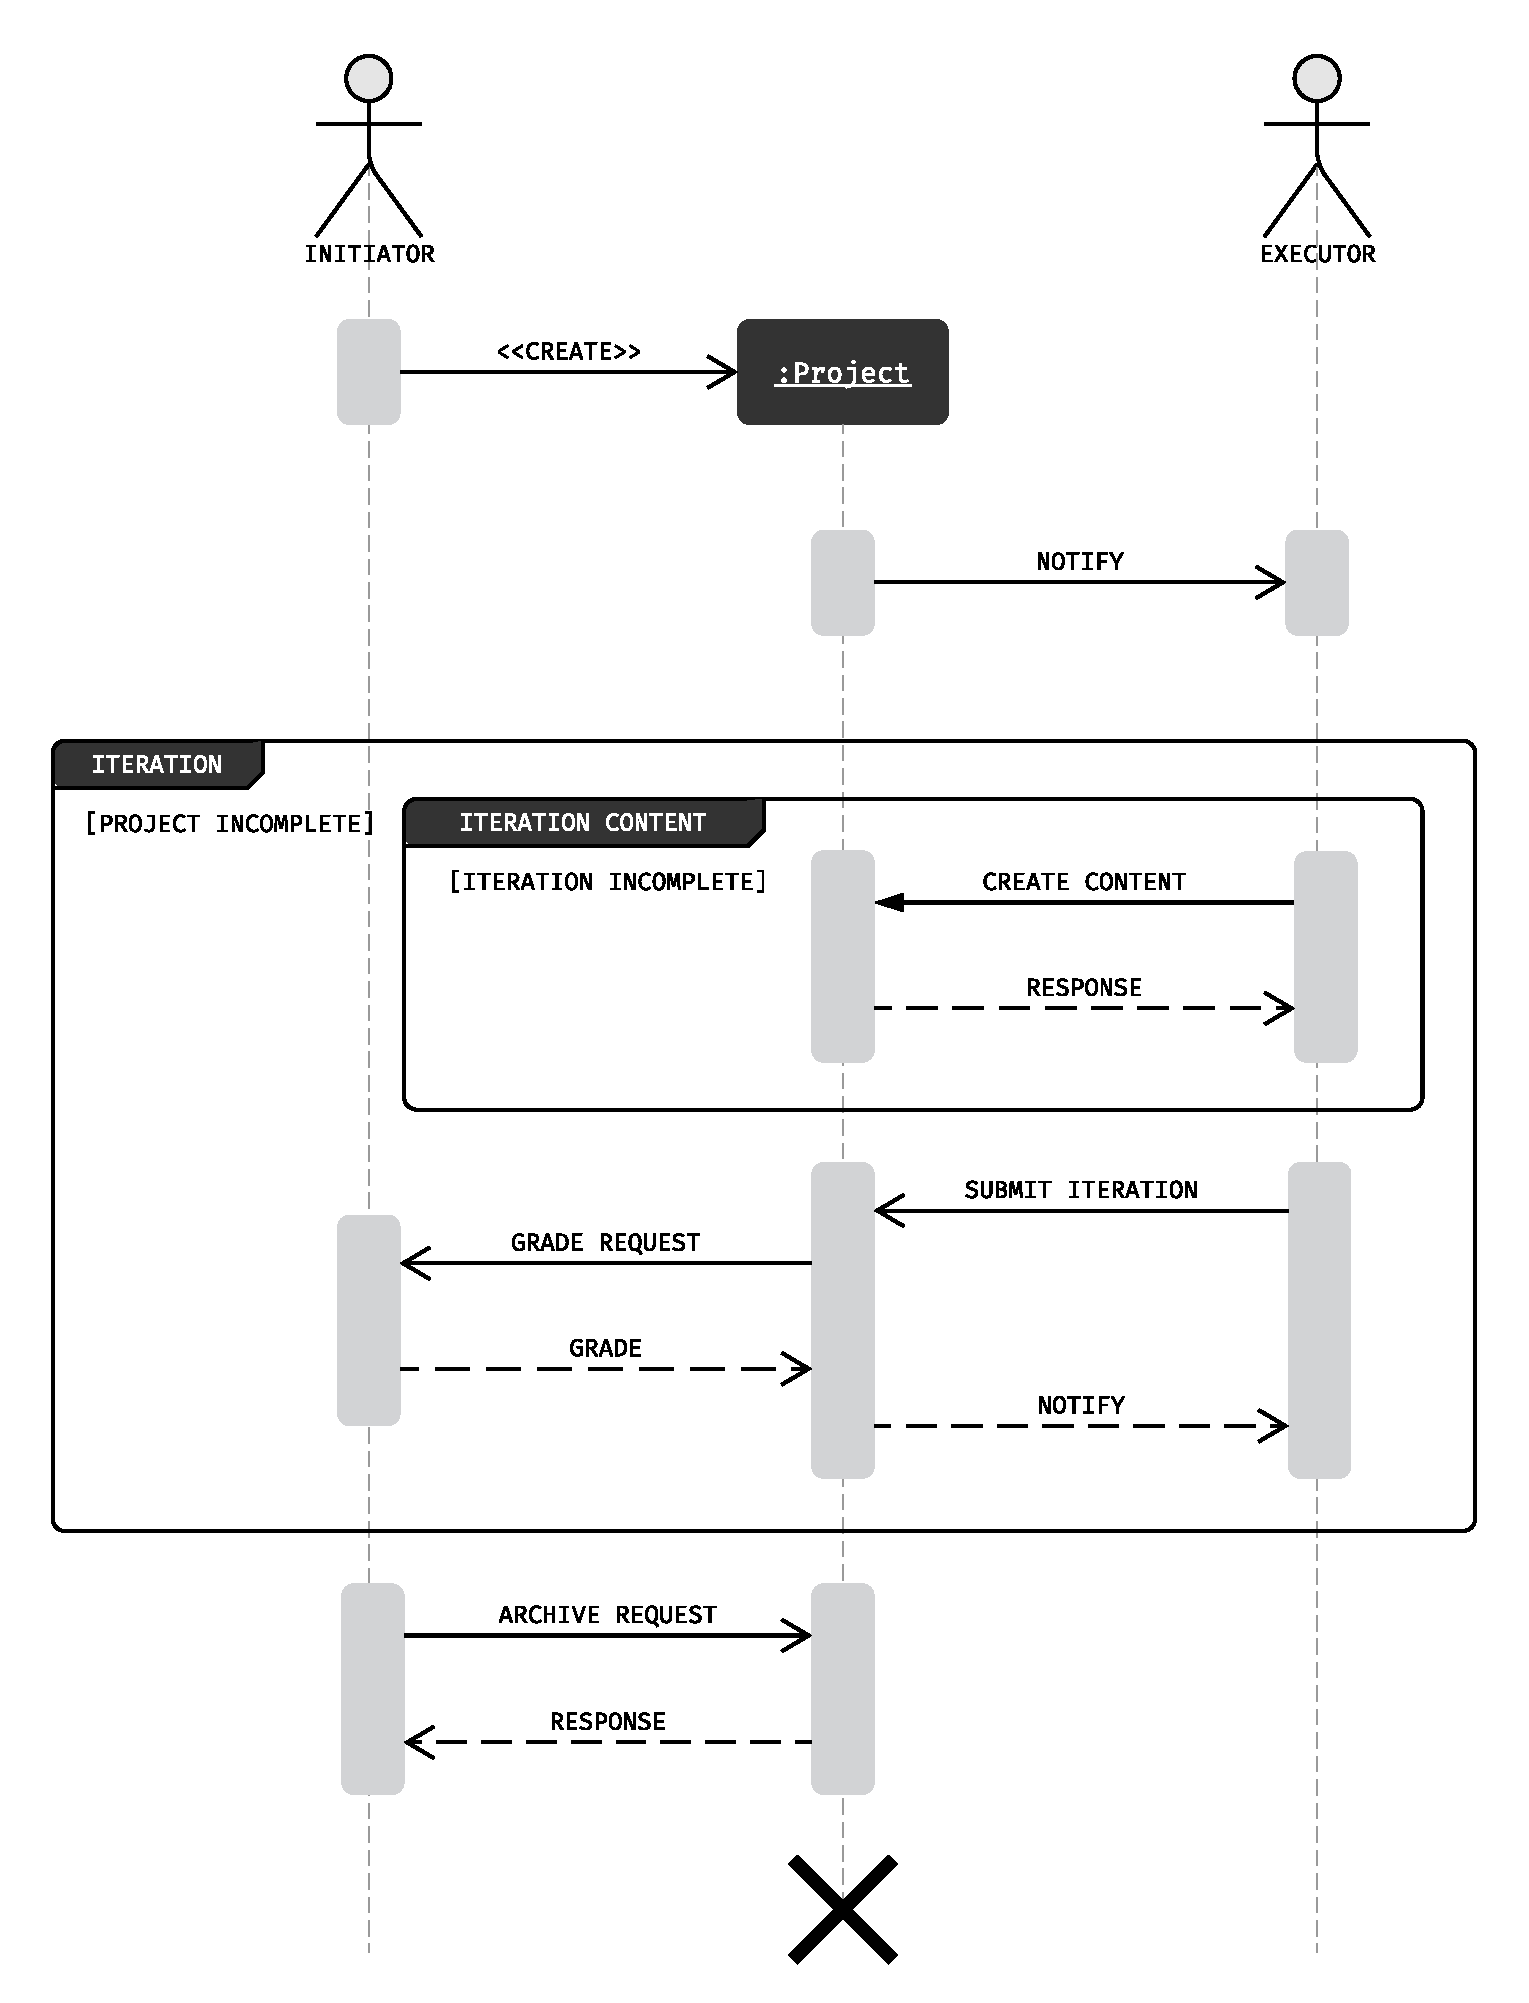
\includegraphics[max width=\textwidth]{assets/dia-seq-study-project-lifecycle}
   \caption[Zobecněný životní cycklus projektu]{Zobecněný životní cyklus projektu~\cite{bachelorthesis}}\label{fig:main-communication-cycle}
\end{figure}



\section{Požadavky na systém}\label{sec:spec-req}

Požadavky na \g{IS} z přechozí práce jsou uměle upraveny dle aktuálních potřed, aby vynechaly méně prioriptní věci a byly vhodné pro vývoj na \g{MSA}.



\subsection{Funkční požadavky}\label{subsec:spec-req-func}

\begin{dl}
   \item[FP00] \textbf{Identita uživatelů} – uživatelé se mohou registrovat, přihlásit a vykonávat určité činnosti na základě přidělených práv.
   \item[FP01] \textbf{Globální role} – práva uživatelů jsou přidělována na základě rolí, administrátor systému má má neomezený přístup a má právo změnit roli uživatele.
   \item[FP02] \textbf{Uživatelská data} – aplikace umožňuje uživatelům prohlížet si svoje data a v případě nutnosti odstanit referenci na jejich osobu (odstranit účet).
   \item[FP03] \textbf{Upozornění} – aplikace posílá uživatelům relevantní upozornění na základě změn v \g{IS}.
   Uživatel takové upozornění může označit jako přečtenou/nepřečtenou, nebo odstranit.
   \item[FP04] \textbf{Projekt – životní cyklus} – aplikace umožňuje uživatelům zakládat projekty s definováním detailních interních informací.
   Projekt může být následně upravován až do jeho zániku (permanentní odstranění), nebo pozastavení (archivování na dobu neurčitou).
   Projekt lze z archvívu obnovit a pokračovat v úpravách.
   \item[FP05] \textbf{Projekt – správa dat} – aplikace umožňuje každému projektu definovat veřejná, skrytá (pouze pro účastníky projektu) a volitelně skrytá data.
   \begin{ul}
      \item {\textbf{Veřejná} – kategorie, název, věřejný popis, cleny týmu, tagy, status archivace.}
      \item {\textbf{Skrytá} – iterace a úkoly, interní popis, snímky iterací a ohodnocení.}
      \item {\textbf{Volitelně skrytá} – vakantní pozice, obsah.}
   \end{ul}
   \item[FP06] \textbf{Projekt – kategorie a tagy} – aplikace umožňuje každému projektu definovat kategorie a tagy, dle kterých se dá vyhledávat.
   Seznam kategorií je spravován administrátory \g{IS}.
   V případně prázdné ketegorie, se dá odstranit.
   \item[FP07] \textbf{Projekt – tým a role} – v rámci každého proejktu každý uživatel má určitou roli, která mu přiděluje oprávění pro prohlížení/úpravu projektu.
   \begin{ul}
      \item {\textbf{Vedoucí} – neomezený přístup k projektu, spravuje všechny detaily projektu (role, uživatele, popis, tagy apod.). Prvním vedoucím se stává uživatel, jenž projekt založil. Vedoucí může povolit/zakázat roli Náveštěvník a definovat nové role v týmu, které budou mít stejná práva, jako role Spolupracovník.}
      \item {\textbf{Spolupracovník} – podílí se na tvorbě obsahu projektu, nezasahuje do interní správy projektu (název, přístupová práíva apod.).}
      \item {\textbf{Návštěvník} – může prohlížet detaily projektu.}
   \end{ul}
   Z projektu lze odejít, pokud se nejedná o posledního uživatele s rolí Vedoucí.
   Vedoucí může povolit/zakázat nábor uživatelů na role, u kterých je uvedena kapacita.
   Pokud má uživatel status důveryhodného, může přidávat členy týmu bez jejich souhlasu.
   \item[FP08] \textbf{Projekt – vyhledávání} – aplikace umožňuje vyhledat projekt dle zadaných kriterií.
   \item[FP09] \textbf{Projekt – iterace a úkoly} –
   \item[FP10] \textbf{Projekt – Správa obsahu} – aplikace umožňuje vedoucím a spolupracovníkům tvořit obsah projektu.
   Obssah je členěn do částí – každá část má datovou složku a název interpretu, který bude datovou složku zpracovávat do vizuální podoby.
   Každá část může označovat jeden, či více úkolů za splněné.
   \item[FP11] \textbf{Projekt – snímky iterací} – stav obsahu projektu se da zafixovat a odeslat k ohodnocení u konkrétní iterace.
   \item[FP12] \textbf{Projekt – důvěryhodnost} – projekt je označen za důvěryhodný, pokud alespoň jeden z vedoucích je důvěryhodný.
\end{dl}



\subsection{Nefunkční požadavky}\label{subsec:spec-req-common}
\begin{dl}
   \item[FP00] \textbf{Veřejné \g{API}} – aplikace bude nabízet veřejné \g{API} s dokumentací pro vývoj aplikací.
   \item[FP01] \textbf{Dokumentace} – součástí \g{IS} je uživatelská a vývojářská dokumentace.
   \item[FP02] \textbf{Rozšiřitelnost} – aplikace je připůsobena dalšímu rozvoji a umožňuje škálovat jednotlivé části fukcionality dle zátěže.
   \item[FP03] \textbf{Uživatelské rozhraní} – uživatelské rozhraní je ve webové podobě a podporuje prohlížeč Google Chrome.
   Mobilní rozhraní není potřeba.
   \item[FP04] \textbf{Jazykové verze} – rozhraní je připraveno pro překlad do dalších jazyků.
   \item[FP05] \textbf{Úložiště dat projektů} – úložiště dat projektů bude možné konfigurovat před prvním spuštěním \g{IS}.
   Výměna úložiště se zachováním údajů během provozu \g{IS} není nutná.
\end{dl}





\TODO{Napsat testovací scénáře pro testování funkčnosti, viz kapitola Testování}

   \chapter{Analýza a implementace serverové části}\label{ch:server}


Vzhledem ke změněým požadavkům a potřeby změny architektury bylo rozhodnuto přepsat celou implementaci serverové části od začátku.
Původní zdrojový kód bude sloužit pouze jako inspirace pro realizaci některých funkcionalit.



\section{Databáze a migrace}\label{sec:server-db}



\section{Sestavování balíčku a kontejnerizace}\label{sec:server-compile}

Vzhledem k používaným technologiím zdrojový kód aplikací nelze spouštět bez předchozího zpracování.
TypeScript, jako samostatný jazyk, vyžaduje transpilaci kódu do JavaScript přes vhodný nástroj, například \h{tsc}.
Dle výchozího chování vytváří vedle každého rozpoznaného \h{.ts} souboru jeho transpilovanou kopii, importované a exportované části se neslučují.
V takovém stavu se \h{.js} soubory již dají spouštět za pomocí nástroje \h{node} (Node.js).

Obdobného chování, ale již bez explicitního transpilování, lze dosáhnout s pomocí nástroje \h{ts-node}.
Balíček \h{ts-node} je dle jednoho z autorů připraven pro produkční prostředí a program může být spuštěn bez dopadu na výkon~\cite{tsnodeprod}.
Tento výsledek by se dal považovat za uspokojivý, avšak ne v případě kontejnerizace.

Vzhledem k vnějším závislostem z adresáře \h{node\_modules}, které v obou případech zůstávají zachovány, bude nutné ponechávat celý adresář po \h{build} fázi v Docker obrazu.
To může mít za následek nevhodnou velikost výsledného kontejrenu, v daném projektu by to znamenalo přibližně \TODO{2GB} zbytečných dat (vývojářské nástroje, zdrojové kódy knihoven apod.) pro každou aplikaci.
V případě mohutnějších \g{MS} by dané číslo mohlo být mnohem větší a přidalo by negativní dopad na požadavky parametrů serverů.

Jako řešení se nabízí selektivní kopírování potřebných souborů z \h{node\_modules} adresáře do Docker obrazu.
Z tohoto důvodu do sestavování \g{MS} byl přidán nástroj \h{webpack} a další, potřebné pro vývoj, balíčky.
Tímto zásahem se přišlo o jednoduchost transpilace – \h{webpack} přebral úkol předzpracování \h{.ts} souborů, ale získalo se mnohem ohebnější prostředí.
Výstup vytvářený \h{webpack} je \h{.js} soubor, jenž nepotřebuje vnější závislosti a je soběstačny – zahrnuje v sobě kopie všech závislostí a potřebuje pouze vnější JavaScript interpet, který se získává z rodičovského Docker obrazu.

Lokální vývoj s tímto nastavením nepotřebuje žádnou logiku navíc.
Pro účely vývoje se přidal nástroj \h{nodemon}, jenž umožňuje hot-reloading\footnote{Hot-reloading je automatické přenačtení a spuštění programu, které se provádí po každé změně kódu.}.

Ve výsledku se každá \g{MS} začala sestavovat s pomocí \h{webpack}, výstupem je samostatná sada transpilovaných a minifikovaných souborů, jež je použita v druhé fázi sestavování.
Dockerfile konfigurace je detailně popsaná v kapitole \nameref{ch:deployment}.

   \chapter{Analýza a implementace klienské části}\label{ch:client}

Daná kapitola se věnuje analýze a implementaci klienské části na základě bodů uvedených v kapitole \enquote{Analýza předchozí práce}.
Implicitně, bez textového rozboru, budou odbaveny méně komplexní záležitosti.
Implementačně zajímavé prvky budou naopak popsány v následujících podkapitolách.



\section{Architektura}\label{sec:client-arch}

Vzhledem k aplikaci menšího rosahu a bez zátěžově nevyvážených komponent, není nutné implementovat strukturu podobnou mikroservisní klientné aplikace.
Základ je převzat z bakalářské práce – řešení založené na frameworku Next.js s využitím \g{SSG} a \g{SSR}.
Obsash projektů i nyní bude tvořen za pomocí načítání externích \h{.js} souborů s valstní inicializací, ale samotná realizace musí být upravena pro větší izolaci jednotlivých částí obsahu.

\section{Zdokonalení struktury a funkcionality}\label{sec:client-improve}




\begin{dl}
   \item[Vizuální vzhled rozhraní] –
   \item[Podpora internacionalizace a lokalizace] – V používané knihovně Next.js od verze 10.0.0 je přidaná podpora internacionalizace – možnost přidat seznam lokalizovaných prvků a výchozí lokalizaci, o zbytek (směrování apod.) se stará knihovna~\cite{nextjsi18n}.
   \item[React hooks] –
   Přechod na modernější způsob zápisu React komponent s využitím \enquote{React hooks} nebyl nutný, nicméně v rámci přepisování větší části klietské aplikace bylo rozhodnuto použít nový způsob zápisu.
   Přineslo to (v porovnáním s původním kódem) výrazné snížení objemu kódu a zlepšení přehlednosti.

   Bylo experimentálně ověřeno, že rozdíl z hlediska rychlosti zpracování není tolik výrazný.
   Rozdíl se objevuje především v objemu generovaného kódu.
   V případě funkcionální komponenty je objem několikanásobně menší, než v případě class komponenty.~\cite{reacthooksdiff}

   \item[Nepříznivé scénáře \g{API} dotazů] – \TODO{axios interceptors}
\end{dl}





\subsection{Autentizace}\label{sec:client-auth}

Větší rozsah změn se dotknul autentizaci a autorizaci uživatele v aplikaci.
Částečně přizpůsobený OAuth 2.0 se nahradil běžnou, nezávislou implementací access/refresh tokenů pro přístup na web.
Zjednodušil se tím postup registrace a přihlašování.
Za veškerou logiku získávání a obnovování tokenů

\TODO{popsat implementaci access a refresh tokenu s pomoci axios}



\section{Interprety obsahu}\label{sec:client-interpret}

\TODO{popsat novou implementaci integrace interpretů}

\TODO{doplnit sekvencni diagram komunikace se servery}


U klientských mikrobalíčků by existovala
- inkapsulace CSS
- inkapsulace JS - zadny, nebo dohodnuty global space





\subsection{Kontejnerizace a zátěž}\label{sec:client-container}

\TODO{obdobně, jako u serverových \g{MS}, popsat klíčové prvky kontejnerizace.}

   \chapter{Testování}\label{ch:testing}


Popsané znalosti jsou aplikovány v rámci implementovaného \g{IS} s vhodně vybraným rozsahem pokrytí.

\section{Serverová část}\label{sec:testing-server}

Serverové části se týká především jednotkové, integrační a funkční testování.



\subsection{Jednotkové testování}\label{subsec:testing-server-unit}



\subsection{Integrační testování}\label{subsec:testing-server-integration}



\subsection{Funkční testování}\label{subsec:testing-server-functional}

\section{Klientská část}\label{sec:testing-client-app}

Na straně klinsta se bude provádět testování

\subsection{Jednotkové testy}\label{subsec:testing-client-app-unit}

Obdobně, jako v případě každé \g{MS} pro jednotlivé části implementace byly napsány jednotkové testy, které se prováděly buď manuálně, nebo automaticky (vynuceně) během každé \enquote{push} akce v \h{git}.
Vynucená kontrola byla řešena s pomocí \h{git} hooks.

Následně byla automatizována kontrola základních interakcí a průchodů \g{MS} pomocí \TODO{Vybrat nástroj} (viz podkapitola Funkční testování).
Ná závěr byla provedeno akceptační testování (viz podkapitola Uživatelské akceptační testování).



\subsection{Funkční testování}\label{subsec:testing-client-app-functional}


\subsection{Uživatelské akceptační testování}\label{subsec:testing-client-app-acceptance}
Poslední fází je \g{UAT}, neboli uživatelské akceptační testování.
Daný typ testování se stěží nahrazuje automatickou formou, protože jde zejména o ověřování splněnosti požadavků klientem.


   \chapter{Kontejnerizace a nasazení}\label{ch:deployment}

Pro kontejnerizaci klientské i serverové části byl použit Docker, alternativní nástroje nebyly zvažovány.


%   \chapter{Style Guide}\label{styleguide}

\section{Section 1}
\subsection{Section 2}

\begin{REFACTOR}
	Lorem ipsum dolor sit amet, consectetuer adipiscing elit. Aenean commodo ligula eget dolor. Aenean massa \footnote{Lorem ipsum dolor.}.
\end{REFACTOR}


Nulla imperdiet imperdiet enim, et tristique risus. Fusce eu neque a ipsum aliquam viverra. Praesent sed vehicula \lfbox{metus}, sed sodales orci. Sed \verb|dolor| sit amet amet, consectetuer ${5} \over {4}$ adipiscing eleifend \gls{MSA}.

$$\int {\gamma^n + y^n } dx = { 5 \over 8}$$

\begin{figure}\centering
   
\includegraphics[max width=\textwidth]{cvut-logo-bw-en.pdf}
   \caption[List label 1]{Caption label 1}\label{pic:ctulogo}
\end{figure}


\begin{figure}\centering
   \begin{minted}{javascript}
// Dependencies
require('Styles/index.scss');
const Application = require('Core/Application.class');
// Application
global.app = new Application();
app.init(x <= 5);
app.getRouter().refresh();
   \end{minted}
   \caption[List example of JS code]{Caption example of JS code}\label{code:jsexample}
\end{figure}


\begin{table}\centering
   \begin{tabular}{|c|r|r|}
      \hline \textbf{Method} & \textbf{Data to encode} & \textbf{Encoded data} \\\hline
      RLE 1 & \textit{babaaaaabbbaabbbba11aaa} & \textit{$1$b$1$a$1$b$5$a $3$b$2$a$4$b$1$a $2$1$3$a} \\\hline
      RLE 2 & \textit{babaaaaabbbaabbbba11aaa} & \textit{bab$@5$a$@3$ baa$@4$ba1 1$@3$a} \\\hline
   \end{tabular}
   \caption[List label 1]{Caption label 1}\label{tab:example1}
\end{table}

\begin{table}\centering
   \begin{tabular}{| l | c r |}
      \hline
      1 & 2 & 3 \\
      4 & 5 & 6 \\
      7 & 8 & 9 \\
      \hline
   \end{tabular}
   \caption[List label 2]{Caption label 2}\label{tab:example2}
\end{table}


\subsection{Subsection}
Lorem ipsum  elit venenatis \ref{code:example}.

\begin{dl}
	\item[NEC] natoque penatibus,
	\item[Venenatis] enim justo rhoncus.
\end{dl}

\begin{ol}
	\item {Sociis natoque penatibus}
\end{ol}

\begin{ul}
	\item In enim justo, rhoncus ut imperdiet a venenatis.
\end{ul}



   \begin{conclusion}
      Na základě získaných znalostí a zkušeností nelze říct, že nějaká z architektur je lepší, nebo horší, než ostatní.
Každá má svůj účel a svoje potřeby, může být různě kongurována a upravována dle situací, ve kterých se nechází.

\g{MSA} najde svoje uplatnění zejména v extrémě komplexních, nebo extrémě nerovnoměrně zatížených systémech.
Uplatnění \g{MSA} v této práci pro implementaci informačního systému nebyla vhodná z hlediska rozsahu práce.
Systém nebyl dostatečně komplexní a jeho vytížení nebylo předem známo.

   \end{conclusion}

   \bibliographystyle{csn690}
   \bibliography{bibliography}

   \appendix
   % glossary
\printglossary[nogroupskip=true,style=index]

% media description


\chapter{Obsah přiloženého média}

Vizualizace struktury souborů na přiloženém médiu.

\begin{figure}
   \dirtree{%
      .1 README.txt\DTcomment{soubor s popisem}.
      .1 src\DTcomment{adresář se zdrojovými soubory}.
      .2 applications\DTcomment{adresář se zdrojovými soubory aplikace}.
      .2 thesis\DTcomment{adresář se zdrojovými soubory textu}.
      .1 text\DTcomment{adresář s textem diplomové práce}.
      .2 thesis.pdf\DTcomment{diplomová práce v PDF formátu}.
      .1 resources\DTcomment{adresář s přílohami}.
   }
\end{figure}


\end{document}
